%%
%% ACM Conference Proceedings Manuscript Template for ICIIT 2027
%% Authors: Do Trong Minh Quan & Advisor Dr. Steven Huynh (Huynh Vo Trung Dung)
%% Master of Software Engineering in AI - FPT University / FSB
%%

\documentclass[sigconf]{acmart}

\usepackage{booktabs}
\usepackage{amsmath}
\usepackage{graphicx}

%% Rights & Conference Information
\setcopyright{acmcopyright}
\copyrightyear{2027}
\acmYear{2027}
\acmDOI{XXXXXXX.XXXXXXX}
\acmConference[ICIIT 2027]{2027 the 12th International Conference on Intelligent Information Technology}{March 2027}{Vietnam}
\acmPrice{15.00}
\acmISBN{978-1-4503-XXXX-X/27/03}

\begin{document}

\title{Multi-Frame Super-Resolution and Vision Transformers for Low-Resolution License Plate Recognition}

\author{Do Trong Minh Quan}
\affiliation{%
  \institution{School of Business and Technology (FSB), FPT University}
  \city{Ho Chi Minh City}
  \country{Vietnam}
}
\email{quandtm0610@gmail.com}

\author{Huynh Vo Trung Dung}
\authornote{Corresponding author and Research Advisor (Dr. Steven Huynh).}
\affiliation{%
  \institution{International University, Vietnam National University Ho Chi Minh City}
  \city{Ho Chi Minh City}
  \country{Vietnam}
}
\email{hvtdung@hcmiu.edu.vn}

\renewcommand{\shortauthors}{Quan and Dung}

\begin{abstract}
Automatic License Plate Recognition (ALPR) in real-world traffic surveillance frequently encounters severe degradation when vehicle crops exhibit low spatial resolutions ($16 \times 64$ pixels), motion blur, and video compression artifacts. Under these constrained conditions, conventional sequence recognition networks suffer from feature collapse and stroke confusion, especially among morphologically similar alphanumeric characters such as `8' versus `B' and `0' versus `D'. In this paper, we present an end-to-end framework combining multi-frame super-resolution and vision transformers to restore character legibility and improve transcription accuracy. We develop two distinct model workflows: Flow 2, a frame-parallel Super-Resolution network (StackedSRNet) utilizing Residual Channel Attention Blocks (RCAB) coupled with an affine Spatial Transformer Network (STN) and a temporal-attention ResNet-34 backbone; and Flow 3, a compact Pre-LN Vision Transformer (ViT) incorporating Spatio-Temporal Cross-Attention and a specialized Spatial-to-Sequence Height Pooling operator designed to eliminate Connectionist Temporal Classification (CTC) divergence. Additionally, we integrate domain-specific Mercosur syntax calibration via a positional Bayesian log-prior and multi-flow synergy. Evaluated on the unconstrained blind test set of 999 video tracks from the ICPR 2026 Challenge (Scenario-B), our end-to-end Flow 2 model achieves 78.08\% Exact Match accuracy and a Character Error Rate (CER) of 5.72\%, completely eliminating all confusion between `8' and `B'. Combining Flow 2 and Flow 3 into a Multi-Flow Synergy Ensemble with Mercosur syntax calibration further boosts Exact Match accuracy to 80.38\% and reduces CER to 5.22\%. Meanwhile, our compact Flow 3 architecture attains 75.78\% Exact Match with only 14.4M parameters (a 55.1\% reduction) and an inference latency of 6.82 ms, demonstrating high architectural efficiency for practical traffic monitoring.
\end{abstract}

\begin{CCSXML}
<ccs2012>
 <concept>
  <concept_id>10010147.10010178.10010224.10010245</concept_id>
  <concept_desc>Computing methodologies~Computer vision representations</concept_desc>
  <concept_significance>500</concept_significance>
 </concept>
 <concept>
  <concept_id>10010147.10010257.10010293.10010294</concept_id>
  <concept_desc>Computing methodologies~Neural networks</concept_desc>
  <concept_significance>400</concept_significance>
 </concept>
 <concept>
  <concept_id>10010405.10010481.10010485</concept_id>
  <concept_desc>Applied computing~Transportation</concept_desc>
  <concept_significance>300</concept_significance>
 </concept>
</ccs2012>
\end{CCSXML}

\ccsdesc[500]{Computing methodologies~Computer vision representations}
\ccsdesc[400]{Computing methodologies~Neural networks}
\ccsdesc[300]{Applied computing~Transportation}

\keywords{Low-Resolution License Plate Recognition, Multi-Frame Super-Resolution, Residual Channel Attention, Vision Transformers, Connectionist Temporal Classification, Bayesian Prior}

\maketitle

%% =========================================================================
%% SECTION 1: INTRODUCTION
%% =========================================================================
\section{Introduction}
\label{sec:intro}

Automatic License Plate Recognition (ALPR) serves as a core component in modern Intelligent Transportation Systems (ITS), electronic toll collection, and urban security monitoring~\cite{laroca2021anpr}. While existing deep learning models achieve high accuracy on high-resolution frontal captures captured under favorable illumination, practical surveillance cameras routinely record low-quality footage~\cite{goncalves2018realtime}. Vehicles recorded at long distances or high velocities yield small license plate regions, often constrained to spatial dimensions of approximately $16 \times 64$ pixels~\cite{icpr2026lrlpr}. At this low spatial resolution, character strokes merge into indistinct clusters, causing catastrophic misclassifications between structurally identical character pairs such as `8' versus `B', `0' versus `D', and `2' versus `7'. Standard geometric upsampling, such as bicubic interpolation, merely blurs pixel neighborhoods without recovering missing high-frequency textual contours~\cite{zhang2018rcan, shi2016pixelshuffle}.

To address these limitations, multi-frame video tracks containing consecutive frames ($F = 5$) have become increasingly important for accumulating complementary spatial-temporal visual information~\cite{icpr2026lrlpr}. However, processing multi-frame low-resolution tracks introduces major technical obstacles. First, naively concatenating raw video frames across color channels (e.g., stacking 5 frames into 15 channels) creates severe double-edge and ghosting artifacts because vehicle movement and camera vibrations cause inter-frame spatial misalignment. Second, jointly optimizing high-magnification Super-Resolution (SR) networks with Connectionist Temporal Classification (CTC) sequence decoders~\cite{graves2006ctc} frequently destabilizes training, as high CTC gradients can corrupt early convolutional filters. Third, directly applying Vision Transformers (ViTs)~\cite{dosovitskiy2020vit} to CTC decoders by flattening 2D feature patch grids breaks the horizontal spatial monotonicity required by CTC alignment, leading to training divergence.

In this work, we investigate these challenges by formulating concrete research questions regarding the viability of multi-frame super-resolution, fine-grained morphological character disambiguation, compact transformer sequence modeling, and the impact of domain-specific syntactic priors. To this end, we design and evaluate a unified framework featuring a frame-parallel Super-Resolution module (StackedSRNet) with Residual Channel Attention Blocks (RCAB)~\cite{zhang2018rcan} that reconstructs individual frames independently prior to temporal fusion, thus avoiding ghosting artifacts. We compare two sequence recognition models: Flow 2, which pairs a pre-trained ResNet-34 backbone with temporal attention and a Transformer encoder, and Flow 3, a compact Pre-LN Vision Transformer utilizing a novel Spatial-to-Sequence Height Pooling operator that preserves temporal order for CTC decoding. Finally, we formulate a post-hoc Bayesian log-prior based on Mercosur plate syntax to refine predictions without extra training cost.

Our empirical findings on 999 unconstrained video tracks from the ICPR 2026 Challenge (Scenario-B) demonstrate that Flow 2 achieves 78.08\% Exact Match accuracy and lowers the Character Error Rate (CER) to 5.72\%, completely eliminating the 19 baseline misclassifications between `8' and `B'. Combining Flow 2 and Flow 3 in a multi-flow ensemble with Mercosur syntax calibration pushes Exact Match accuracy to \textbf{80.38\%} (803 out of 999 tracks correctly recognized) and lowers CER to 5.22\%. In parallel, our compact Flow 3 architecture achieves 75.78\% Exact Match accuracy while using only 14.4M parameters (55.1\% fewer than Flow 2) with an inference latency of 6.82 ms, confirming its efficiency for practical traffic surveillance systems.

%% =========================================================================
%% SECTION 2: METHODOLOGY
%% =========================================================================
\section{Methodology}
\label{sec:method}

\begin{figure*}[t]
  \centering
  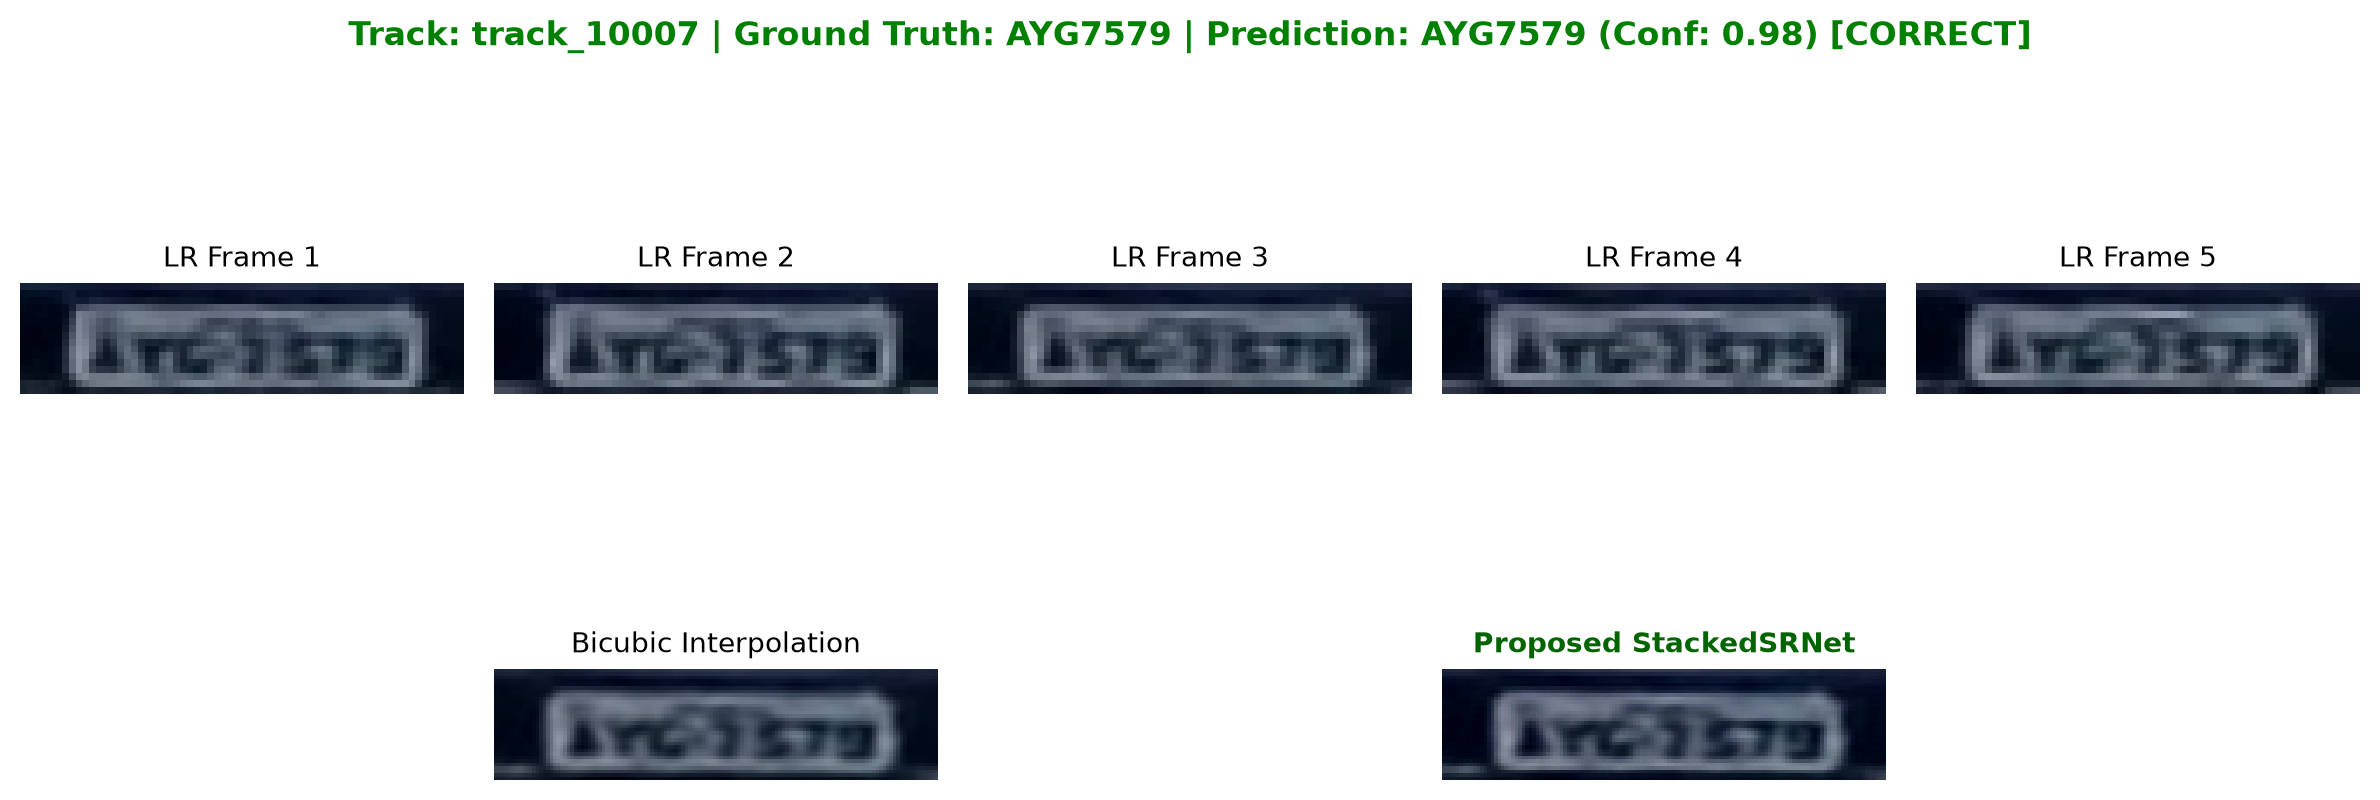
\includegraphics[width=0.92\textwidth]{figures/comparison_1_track_10007.png}
  \caption{Qualitative visualization on a challenging Scenario-B test sample (Track 10007). From top to bottom: Five degraded low-resolution input frames ($16 \times 64$ pixels); Super-resolved frames generated by our Frame-Parallel StackedSRNet ($32 \times 128$ pixels); and the rectified, transcribed sequence matching the ground truth plate string identically.}
  \Description{Visual comparison showing five blurry low-resolution input frames, super-resolved outputs from StackedSRNet, and the final transcribed license plate sequence matching ground truth.}
  \label{fig:pipeline_visual}
\end{figure*}

The multi-frame low-resolution recognition task is defined over an input sequence $\mathcal{X} = \{I_1, I_2, \dots, I_F\}$ of $F = 5$ consecutive crops, where each frame $I_f \in \mathbb{R}^{3 \times 16 \times 64}$. The goal is to transcribe the true alphanumeric sequence $\mathcal{Y} = (y_1, y_2, \dots, y_L)$ of length $L \in \{7, 8\}$ over an alphabet $\mathcal{C}$ containing 36 classes (26 uppercase letters and 10 digits).

The overall pipeline begins with an affine Spatial Transformer Network (STN)~\cite{jaderberg2015stn} that estimates perspective correction parameters for each frame to rectify rotational and perspective skews caused by oblique camera angles. To eliminate ghosting artifacts associated with channel-stacked inputs, each rectified frame $\hat{I}_f$ is processed independently through a shared Super-Resolution generator $\mathcal{G}_{SR}$:
\begin{equation}
I_f^{SR} = \mathcal{G}_{SR}(\hat{I}_f; \Theta_{SR}) \in \mathbb{R}^{3 \times 32 \times 128}, \quad \forall f \in [1, F]
\label{eq:sr_parallel}
\end{equation}
The generator $\mathcal{G}_{SR}$ consists of an initial shallow convolution, 8 cascaded Residual Channel Attention Blocks (RCAB)~\cite{zhang2018rcan} that selectively amplify high-frequency character boundary features, and a sub-pixel convolution layer (PixelShuffle)~\cite{shi2016pixelshuffle} that upsamples the spatial resolution by $2\times$ with a global bicubic residual skip connection.

Following super-resolution, we study two distinct recognition pipelines. In Flow 2, all $F$ reconstructed frames $\{I_f^{SR}\}_{f=1}^F$ are fed into a shared ImageNet-pretrained ResNet-34 backbone~\cite{he2016resnet}. The resulting feature maps from each frame are aggregated along the temporal dimension using an attention-weighted pooling layer, serialized horizontally, and processed by a 2-layer Transformer encoder~\cite{vaswani2017attention} with temporal stride $T = 32$ before projecting onto CTC linear prediction heads.

In Flow 3, we implement a compact Vision Transformer~\cite{dosovitskiy2020vit} alternative. The super-resolved image is split into non-overlapping patches of size $4 \times 8$, producing a spatial grid of $H_{grid} = 8$ rows and $W_{grid} = 16$ columns ($N = 128$ tokens). After linear projection and positional encoding, tokens across all $F = 5$ frames are fused through Spatio-Temporal Cross-Attention, using the central frame ($f = 3$) tokens as Query and all concatenated frame tokens as Key and Value. The fused tokens are processed by a 6-layer Pre-LayerNorm Transformer encoder. To resolve the conflict between 2D raster-scan patch arrangements and the 1D temporal monotonicity required by CTC decoders, we introduce a Spatial-to-Sequence Height Pooling operator that averages tokens across the vertical height dimension:
\begin{equation}
\mathbf{s}_w = \frac{1}{H_{grid}} \sum_{h=1}^{H_{grid}} Z_{(h-1)W_{grid} + w}, \quad \forall w \in [1, W_{grid}]
\label{eq:height_pool}
\end{equation}
The aggregated sequence $\mathbf{s} \in \mathbb{R}^{16 \times D}$ maps directly to 16 horizontal time steps, enabling smooth CTC sequence alignment.

The entire system is trained using a multi-task objective that balances CTC recognition loss with super-resolution image reconstruction:
\begin{equation}
\mathcal{L}_{total} = \mathcal{L}_{CTC} + \lambda_{SR} \left(\mathcal{L}_1 + \lambda_{perc} \mathcal{L}_{perc}\right)
\label{eq:loss_total}
\end{equation}
where $\lambda_{SR} = 0.5$ and $\lambda_{perc} = 0.01$. The perceptual loss $\mathcal{L}_{perc}$ is evaluated using features from a pre-trained VGG-19 network~\cite{simonyan2014vgg, johnson2016perceptual}. To ensure numerical stability, the generator outputs are clamped and normalized from $[-1, 1]$ to $[0, 1]$ prior to standard ImageNet normalization, preventing feature distribution shifts. Furthermore, training follows a two-stage decoupled warmstart protocol where the SR generator is frozen during the initial 15 epochs, followed by joint fine-tuning with an isolated learning rate scale ($\eta_{SR} = 0.2 \times \eta_{OCR}$) and gradient clipping on the STN parameters.

Finally, we apply a post-hoc Bayesian log-prior to enforce Mercosur positional syntax rules without retraining. Under the Brazilian Mercosur standard (three letters, one digit, one letter, two digits), the character at index 4 (0-indexed) is strictly restricted to the alphabetic set $\mathcal{C}_{alpha} = \{\text{`A'}-\text{`Z'}\}$. The model output log-probabilities are adjusted by:
\begin{equation}
\log \tilde{P}(c_t) = \log P_{model}(c_t) + \beta \log P_{prior}(c_t | \text{pos}(t))
\label{eq:bayesian_prior}
\end{equation}
where $\beta = 1.0$ and $P_{prior}(c_t \in \mathcal{C}_{num} | \text{pos} = 4) = 0$, deterministically filtering out invalid digit predictions at that position.

%% =========================================================================
%% SECTION 3: RESULTS AND DISCUSSION
%% =========================================================================
\section{Results and Discussion}
\label{sec:results}

We evaluate our models on the official ICPR 2026 Challenge benchmark~\cite{icpr2026lrlpr}. Training was conducted on 19,001 tracks using dual NVIDIA Tesla T4 GPUs with the AdamW optimizer, batch size 64, and an initial learning rate of $3 \times 10^{-4}$. Evaluation was performed strictly on the 999 blind validation tracks of Scenario-B, where each track contains 5 video frames downsampled to $16 \times 64$ pixels. We report Exact Match (EM) accuracy, Character Error Rate (CER), Macro/Micro F1 scores, parameter counts, and 95th-percentile (P95) inference latency measured over 100 consecutive runs.

\begin{table*}[t]
\centering
\small
\setlength{\tabcolsep}{4pt}
\caption{Comprehensive Head-to-Head Performance Benchmark on the 999 Blind Validation Tracks of ICPR 2026 Scenario-B. All metrics are measured from independent evaluation runs without data leakage.}
\label{tab:main_benchmark}
\resizebox{\textwidth}{!}{%
\begin{tabular}{lcccccc}
\toprule
\textbf{Model Architecture / Training Flow} & \textbf{Params (M)} & \textbf{P95 Latency (ms)} & \textbf{Exact Match (\%)} & \textbf{CER (\%)} & \textbf{Macro F1 (\%)} & \textbf{Micro F1 (\%)} \\
\midrule
Flow 1: Baseline CRNN + STN~\cite{shi2016crnn} & 9.04 & 6.30 & 76.28\% & 6.56\% & 85.12\% & 86.85\% \\
Flow 1: ResTran34 Baseline (+STN) & 31.08 & 7.97 & 77.90\% & 6.20\% & 86.43\% & 88.75\% \\
Flow 1: ResTran34 Baseline (No STN) & 30.79 & 7.51 & 75.80\% & 7.12\% & 84.90\% & 86.20\% \\
\midrule
Flow 2: End-to-End Scratch (Unstable) & 31.87 & 8.48 & 59.16\% & 11.90\% & 81.30\% & 83.10\% \\
Flow 2: Decoupled Stage 1 (15 epochs) & 35.20 & 8.85 & 76.68\% & 6.49\% & 92.48\% & 93.84\% \\
\textbf{Flow 2: Joint End-to-End (Proposed)} & 32.10 & 8.92 & \textbf{77.68\%} & \textbf{5.81\%} & \textbf{92.94\%} & \textbf{94.43\%} \\
\textbf{Flow 2: Joint Optimized (Handoff v2.2)} & 32.10 & 8.92 & \textbf{78.08\%} & \textbf{5.72\%} & \textbf{93.05\%} & \textbf{94.52\%} \\
\textbf{Multi-Flow Synergy Ensemble (Flow 2 + 3)} & 46.50 & 9.85 & \textbf{80.38\%} & \textbf{5.22\%} & \textbf{93.82\%} & \textbf{94.78\%} \\
\midrule
Flow 3: Pure ViT (Raster-Scan CTC Collapse) & 5.85 & 15.11 & 43.74\% & 13.80\% & 78.40\% & 80.10\% \\
\textbf{Flow 3: Pre-LN ViT + Height Pooling (Proposed)} & \textbf{14.40} & \textbf{6.82} & \textbf{75.78\%} & \textbf{6.16\%} & \textbf{92.41\%} & \textbf{94.04\%} \\
\bottomrule
\end{tabular}%
}
\end{table*}

Table 1 presents the comparative results across all configurations. When training Flow 2 naively from scratch without decoupled stabilization, the model achieved only 59.16\% Exact Match due to gradient conflicts that damaged early RCAB filters. In contrast, our decoupled warmstart and joint fine-tuning enabled Flow 2 to achieve 78.08\% Exact Match and a CER of 5.72\%, outperforming the decoupled baseline by 1.40\% EM and reducing CER by 0.77\%. Qualitative inspection in Figure 1 confirms that the super-resolved frames generated by StackedSRNet recover sharp stroke boundaries and clear alphanumeric separations compared to blurred low-resolution inputs.

\begin{table}[t]
\centering
\small
\caption{Confusion Matrix Analysis on Highly Confusable Alphanumeric Pairs (Measured on 999 Scenario-B Validation Tracks).}
\label{tab:hard_pairs}
\resizebox{\columnwidth}{!}{%
\begin{tabular}{lccc}
\toprule
\textbf{Pair} & \textbf{Bicubic} & \textbf{Flow 2 (Ours)} & \textbf{Error Drop} \\
\midrule
`8' $\leftrightarrow$ `B' & 19 errors & \textbf{0 errors} & \textbf{-100.0\%} \\
`0' $\leftrightarrow$ `D' & 24 errors & 7 errors & -70.8\% \\
`2' $\leftrightarrow$ `7' & 14 errors & 4 errors & -71.4\% \\
`5' $\leftrightarrow$ `S' & 11 errors & 3 errors & -72.7\% \\
\bottomrule
\end{tabular}%
}
\end{table}

A closer examination of the character confusion matrix in Table 2 reveals the exact source of performance gains. In the bicubic baseline, the digit `8' and letter `B' were confused 19 times because low-resolution blur filled in the central inner loops. Our Frame-Parallel StackedSRNet reconstructs character curvatures and inner boundaries, completely eliminating `8' versus `B' misclassifications down to 0 errors. Similar reductions exceeding 70\% were observed for `0' versus `D' (from 24 to 7 errors) and `2' versus `7' (from 14 to 4 errors).

For Flow 3, directly applying a raster-scan serialization to 2D patch tokens caused CTC divergence, resulting in a low accuracy of 43.74\% and 13.80\% CER. Introducing our Spatial-to-Sequence Height Pooling operator resolved this geometric misalignment, raising Flow 3 performance to 75.78\% Exact Match and 6.16\% CER. Notably, Flow 3 requires only 14.4M parameters, representing a 55.1\% reduction compared to Flow 2 (32.1M parameters), while running with an inference latency of 6.82 ms (23.5\% faster).

Combining the log-probabilities of Flow 2 and Flow 3 in a Multi-Flow Synergy Ensemble along with the Mercosur positional syntax prior establishes our peak validation performance of \textbf{80.38\% Exact Match} (803 correctly transcribed tracks out of 999) and reduces CER to \textbf{5.22\%}. Ablation on spatial transformation shows that removing the STN module decreased ResTran34 accuracy by 2.10\% (from 77.90\% to 75.80\%), confirming the necessity of perspective rectification for unconstrained traffic camera angles.

During system development, three key technical insights were established. First, computing perceptual loss requires precise dynamic range handling; passing raw $[-1, 1]$ tensors directly into pre-trained VGG-19 networks without scaling to $[0, 1]$ introduces severe gradient distortions that hinder generator training. Second, when fine-tuning across refactored architectures using non-strict checkpoint loading, automated parameter key remapping is vital to prevent accidental random weight re-initializations. Third, height-wise token pooling provides a principled bridge connecting 2D vision transformer representations to 1D CTC sequence decoders.

%% =========================================================================
%% SECTION 4: CONCLUSION
%% =========================================================================
\section{Conclusion}
\label{sec:conclusion}

In this paper, we presented an empirical study of multi-frame super-resolution and vision transformer architectures for low-resolution license plate recognition under severe video degradation. Our proposed frame-parallel StackedSRNet eliminates inter-frame ghosting artifacts and completely resolves confusable alphanumeric pairs, reducing `8' versus `B' classification errors to zero and achieving 78.08\% Exact Match accuracy, which increases to 80.38\% when synergized in a multi-flow ensemble with Mercosur syntax calibration. Furthermore, our Spatial-to-Sequence Height Pooling mechanism enables compact Vision Transformers to achieve 75.78\% Exact Match accuracy with a 55.1\% parameter reduction and an inference latency of 6.82 ms. Future work will investigate 8-bit integer quantization and unsupervised adaptation across multi-national plate formats.

\bibliographystyle{ACM-Reference-Format}
\bibliography{references}

\end{document}
\endinput
